\newpage
\section{Realisering}
\label{realiseringOgTest}

Oppkoblingen ble gjort som vist i den prinsippielle løsningen i figur \ref{fig:diffamp}, hvor strømkliden ble realisert som i figur \ref{fig:CurrentSource}. Modellene og verdiene som ble brukt vises i tabell \ref{tab:komnpomenter}. 

\begin{figure}[!h]
    \centering
    \begin{minipage}[c]{0.4\textwidth}
        \centering
        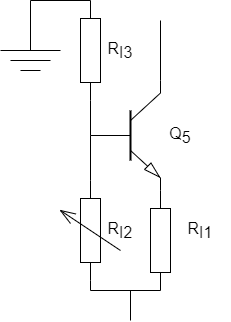
\includegraphics[width=0.6\textwidth]{Bilder/current_source.drawio.png} 
        \caption{Realisert strømkilde.}
        \label{fig:CurrentSource}
    \end{minipage}
    \hfill
    \begin{minipage}[c]{0.5\textwidth}
        \centering
        \begin{tabular}{ |c|c| }
            \hline
            Komponent & Verdi/Produknummer \\ \hline
            \hline
            $Q_1 \& Q_2 \&Q_5$ & BC547A (NPN) \\
            $Q_3 \& Q_4$ & BC557B (PNP) \\
            $R_{I1}$ & $3\text{k}\Omega $ \\
            $R_{I2}$ & $0\Omega - 10\text{k}\Omega$ \\
            $R_{I3}$ & $10\text{k}\Omega$ \\
            \hline
        \end{tabular}
        \\[60pt]
        \caption{Komponenter og verdier brukt i designet.}
        \label{tab:komnpomenter}
    \end{minipage}
\end{figure}

Den oppkoblede kretsen vises i figur \ref{fig:diffamp_realisert}.

\begin{figure}[!h]
    \centering
    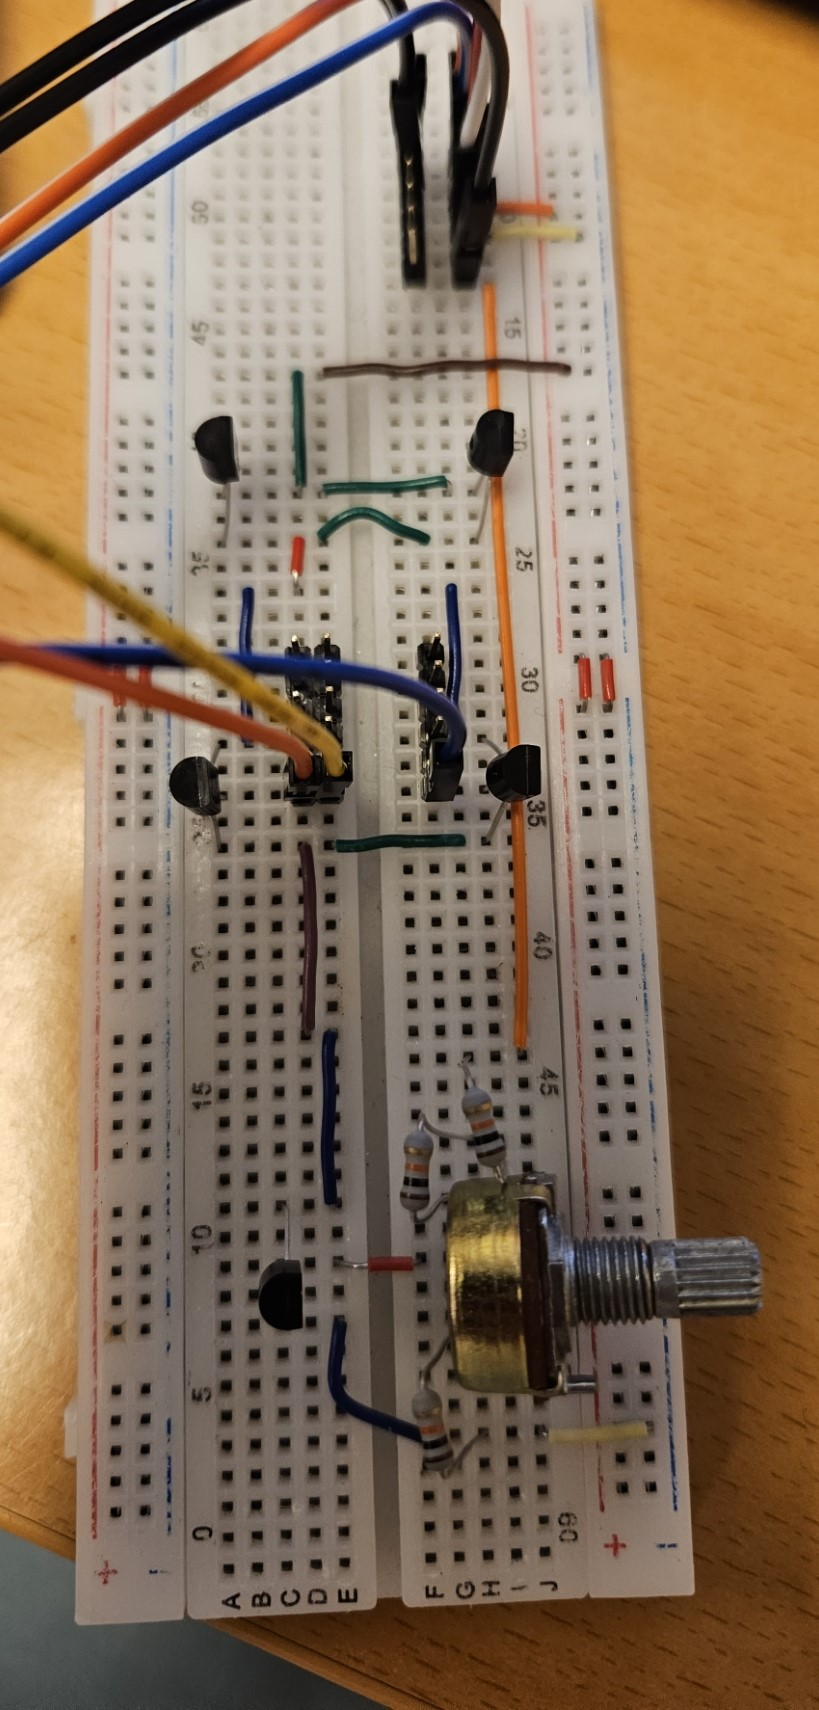
\includegraphics[width=0.4\textwidth, angle=90]{Bilder/feilBilde.jpg}
    \caption{Realisert opperasjonsforsterker}
    \label{fig:diffamp_realisert}
\end{figure}
